\documentclass[11pt,letterpaper]{article}
\usepackage[T1]{fontenc}
\usepackage{lmodern,microtype}
\usepackage[margin=.85in,headheight=15pt]{geometry}
\usepackage{xcolor,booktabs,longtable,array,tabularx,enumitem,amsmath,graphicx,listings,tikz,fancyhdr,titlesec,hyperref,xurl}
\usetikzlibrary{arrows.meta,positioning,fit,shapes.geometric}
\definecolor{navy}{HTML}{16314D}\definecolor{teal}{HTML}{087F83}\definecolor{pale}{HTML}{EDF4F8}\definecolor{muted}{HTML}{536579}
\hypersetup{colorlinks=true,linkcolor=navy,urlcolor=teal,pdftitle={Vendor-Neutral Python Reference Architecture}}
\titleformat{\section}{\Large\bfseries\color{navy}}{\thesection}{.7em}{}
\titleformat{\subsection}{\large\bfseries\color{teal}}{\thesubsection}{.7em}{}
\pagestyle{fancy}\fancyhf{}\fancyhead[L]{\small Agent Harness Engineering}\fancyhead[R]{\small Technical study / v1.0}\fancyfoot[R]{\thepage}
\setlength{\parindent}{0pt}\setlength{\parskip}{5pt}\renewcommand{\arraystretch}{1.18}
\setlist{nosep,leftmargin=*}\newcolumntype{Y}{>{\raggedright\arraybackslash}X}
\newcommand{\src}[1]{\expandafter\nolinkurl\expandafter{\detokenize{#1}}}
\newcommand{\evidence}[1]{\par\smallskip{\small\raggedright\color{muted}\textbf{Source anchor:} #1\par}}
\tikzset{n/.style={draw=navy,rounded corners=2pt,fill=pale,align=center,minimum height=9mm,text width=31mm,font=\small},g/.style={n,draw=teal,fill=teal!7},edge/.style={-Latex,thick,draw=navy},boundary/.style={draw=teal,dashed,rounded corners,inner sep=5pt}}
\lstset{basicstyle=\small\ttfamily,breaklines=true,frame=single,backgroundcolor=\color{pale},columns=fullflexible,showstringspaces=false}
\begin{document}
\begin{titlepage}
\pagenumbering{roman}
\vspace*{1.25in}
{\color{teal}\large AGENT HARNESS COURSE STUDY / 04\par}\vspace{.3in}
{\color{navy}\Huge\bfseries Vendor-Neutral Python Reference Architecture\par}\vspace{.18in}
{\Large Ports and adapters, persistence, deployment and evaluation\par}\vspace{.5in}
\rule{\linewidth}{1pt}\par
\textbf{Source:} Richmond Alake's Harness Engineering for AI Agents course export\par
\textbf{Version:} 1.0 \quad 23 November 2026\par
\textbf{Status:} Technical study; not a production authorization\par
\vfill
The model proposes; the harness validates, governs, executes and records.
\end{titlepage}
\pagenumbering{arabic}
\tableofcontents\clearpage
\section*{Reading note}
This standalone volume belongs to a six-document study of snapshot \src{8a5edab282632443}. Observed source behavior is distinguished from proposed controls. No live application, external provider or sandbox was independently executed. Test files are contract evidence, not independently verified passing results.

\section{Vendor-neutral Python reference architecture}
\subsection{Ports and adapters}
Use Hexagonal Architecture: domain entities and policy are independent of framework, SDK, database and transport. Application services orchestrate typed ports. The model, retrieval, database, MCP, scheduler and sandbox are replaceable adapters. Deploy the API, effect broker, worker/scheduler and audit ingestion under distinct identities; isolate research and candidate-skill evaluation from production effect credentials.
\begin{center}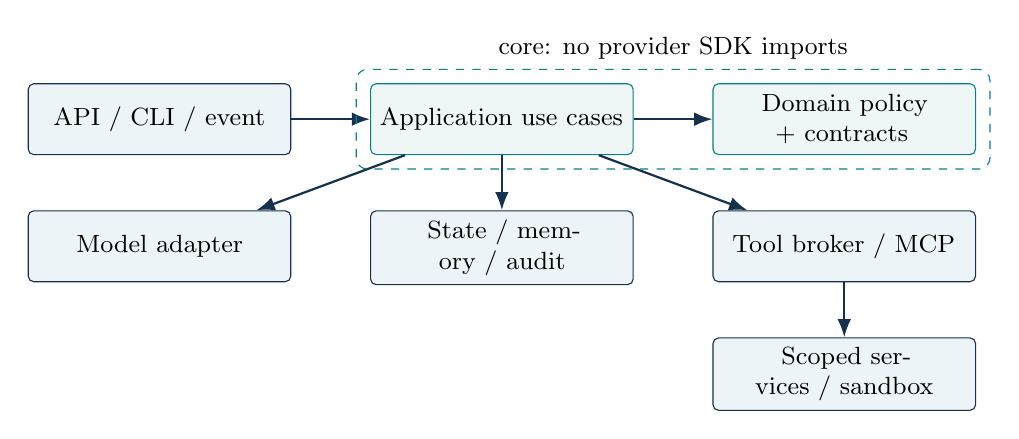
\begin{tikzpicture}[node distance=7mm and 10mm]
\node[n] (api) {API / CLI / event};\node[g,right=of api] (app) {Application use cases};\node[g,right=of app] (domain) {Domain policy + contracts};
\node[n,below=of api] (model) {Model adapter};\node[n,below=of app] (stores) {State / memory / audit};\node[n,below=of domain] (broker) {Tool broker / MCP};
\node[n,below=of broker] (remote) {Scoped services / sandbox};
\draw[edge](api)--(app);\draw[edge](app)--(domain);\draw[edge](app)--(model);\draw[edge](app)--(stores);\draw[edge](app)--(broker);\draw[edge](broker)--(remote);
\node[boundary,fit=(app)(domain),label=above:{\small core: no provider SDK imports}]{};
\end{tikzpicture}\end{center}
\begin{lstlisting}
src/agent_harness/
  domain/        # Principal, Proposal, Effect, PolicyDecision
  application/   # RunTurn, ResumeEffect, PromoteMemory, LearnSkill
  ports/         # Model, Tool, Policy, Memory, State, Audit, Clock
  adapters/      # provider, MCP, database, queue, sandbox, telemetry
  entrypoints/   # HTTP, CLI, worker, scheduler
  composition.py # explicit dependency injection
policy/          # versioned deny-by-default rules
fixtures/        # synthetic data, malicious documents, model scripts
tests/           # contracts, integration, adversarial, fault injection
\end{lstlisting}
\subsection{Core contracts and control loop}
A model returns a discriminated union of FinalAnswer or ToolProposal. Strict validation rejects extra fields, unknown discriminators and wrong types. The host creates run identity; the model cannot set it. A tool descriptor specifies input/output schema, version, scope, risk classification and timeout. The tool adapter receives only authorized, validated arguments and a scoped identity. The effect port separates draft from execute. The state port uses optimistic concurrency or leases; the audit port stores append-only events with correlation IDs and redaction.
\begin{lstlisting}[language=Python]
class ModelPort(Protocol):
    def propose(self, context: Context) -> Proposal | Final: ...
class PolicyPort(Protocol):
    def decide(self, principal: Principal,
               proposal: ValidatedProposal) -> Decision: ...
class ToolPort(Protocol):
    def execute(self, action: AuthorizedAction,
                idempotency_key: str) -> Observation: ...
\end{lstlisting}
Algorithm: authenticate; load state and budget; retrieve scoped evidence; construct trusted instructions and labeled data; call model with deadline; validate; classify policy; deny, execute read, or durably draft and interrupt. Record observations and budget, repeat up to a fixed bound, and persist terminal status. On resume, reload principal and policy, verify the action digest, claim once, execute or reconcile and record. Cancellation terminates new work and revokes unused approvals. Never report an effect as complete on model text alone.
\subsection{Persistence contracts}
\begin{longtable}{>{\raggedright\arraybackslash}p{.24\linewidth}>{\raggedright\arraybackslash}p{.67\linewidth}}\toprule
Record & Required fields and constraints \\\midrule\endhead
Run / checkpoint & tenant, principal, run ID, graph/version, step, deadline, budget, state version; unique run/step \\
Effect & effect ID, run ID, tool/version, canonical argument digest, target, policy, expiry, status, idempotency key; atomic claim \\
Approval & effect ID, digest, approver identity, decision, timestamp, expiry; immutable decision log \\
Memory & owner, type, evidence ID, hash, classification, trust, expiry, version and revocation \\
Skill & name, version, digest, origin evidence, gate result, reviewer, active pointer; one active approved version per scope \\
Trajectory & ordered run events, selected procedure, normalized calls, observed outcome, feedback provenance \\
Audit / usage & event ID, correlation, actor, resource, policy decision, redacted metadata; model usage and configured price version \\
\bottomrule\end{longtable}
\subsection{Execution and deployment decisions}
\begin{tabularx}{\linewidth}{p{.25\linewidth}YY}\toprule
Port & Local learning adapter & Production candidate \\\midrule
Model & Scripted deterministic responder & Any provider via adapter, bounded timeout \\
State & In-memory/SQLite test store & Transactional relational DB with scoped queries \\
Retrieval & Fixture keyword search & Vector/full-text hybrid behind ACL filters \\
Tool & Mock read-only registry & MCP or typed API adapter with scoped token \\
Scheduler & Injected fake clock & Durable queue, lease, retry and dead-letter \\
Sandbox & Fixed operation test double & Isolated job or microVM with egress policy \\
Telemetry & Structured JSON test events & OpenTelemetry-compatible spans and audit sink \\
\bottomrule\end{tabularx}

Deploy read-only first, then mock effects, then approved effects only in a separately authorized application. Network policies deny arbitrary outbound traffic; allow broker-specific domains. Enforce TLS, workload identity, dependency pinning and secret scanning. Use migrations with backward-compatible checkpoints, canary deployments and tested restore. Separate readiness (dependencies and policy loaded) from liveness (process healthy). A release gate must be independent of model-generated judgments.
\subsection{Evaluation, performance and observability}
Measure task success against deterministic or independently graded criteria, forbidden-effect count, approval bypass, audit completeness, retrieval precision/recall, injection detection by class, isolation, recovery and duplicate effects. Record latency percentiles and budget. Price model usage using versioned configured rates:
\[C=(T_f p_f+T_w p_w+T_r p_r+T_o p_o)/10^6.\]
Here fresh, cache-write, cache-read and output tokens are disjoint according to provider accounting; do not double count. Compare harness variants on the same model/version, tool schemas, tasks, budgets and evidence, randomize order and report failures and uncertainty. Cache hit rates are performance indicators, not security indicators.

Part 3's nine-check scorecard has six blocking measures: attacks obeyed (0), unapproved outward actions (0), tasks from quarantine (0), frozen procedure selection (10/10), complete action audit (all), duplicate open tasks per source (0). Three nonblocking reports cover cache-read share, median model seconds and median cost. Extend with tenant isolation, replay, memory poisoning, skill regression, cancellation, dependency outage and restoration tests. Missing mandatory evidence means BLOCKED, not pass; a zero observed count with no trials is inconclusive.
\evidence{Part 3 \src{scorecard.py}, \src{ledger.py}; Part 1 advanced \src{evaluation.py}.}
\section{Architecture decision records and release checklist}
\begin{tabularx}{\linewidth}{p{.19\linewidth}YY}\toprule
ADR & Decision & Consequence \\\midrule
ADR-01 & Model is proposal-only & Host validates and authorizes every tool \\
ADR-02 & Ports over vendor APIs & Adapter effort; framework and provider replaceability \\
ADR-03 & Durable effects separate from checkpoints & More state, reconciliation and audit; safer retry \\
ADR-04 & Memory is scoped evidence & Provenance, retention and cache invalidation needed \\
ADR-05 & Skills are governed artifacts & Shadow tests, immutable version and rollback \\
ADR-06 & Offline-first curriculum & Reproducible labs without provider keys; live parity separately tested \\
\bottomrule\end{tabularx}

Release conditions: all mandatory negative tests pass; no unauthorized external action; identity-scoped storage verified; crash and restore tested; independent evidence reviewed; dependency and secret scans pass; operational runbooks define cancel, revoke, quarantine and reconciliation. No deployment approval is implied by this study.
\section{Source register and limitations}
\begin{itemize}
\item Richmond Alake, \textit{Harness Engineering for AI Agents}, supplied repository export,\newline snapshot \src{8a5edab282632443}; root README, Part 1--3 READMEs, code paths cited throughout. Workshop: \url{https://www.oreilly.com/live-events/harness-engineering-for-ai-agents/0642572381264}.
\item Target curriculum, README and roadmap, inspected 23 November 2026: \url{https://github.com/Notoriousjayy/agent-engineering-curriculum}.
\item Target documentation library, root README and AI technical-documents directory, inspected 23 November 2026: \url{https://github.com/Notoriousjayy/latex-docs}.
\end{itemize}
All figures are original logical reconstructions or proposed design diagrams; they are not copies of source graphics. Vendor-neutral controls, ADRs, acceptance tests and laboratory extensions are recommendations rather than claims about source implementation. Live dependencies, source test outcomes, provider claims, licensing/publication clearance and deployment configuration require separate validation.
\end{document}
